\setcounter{page}{3}

\chapter{Теоретическая часть}



\section{Визуализация базы знаний в Neo4j}

\begin{figure}[h!]
\centering
    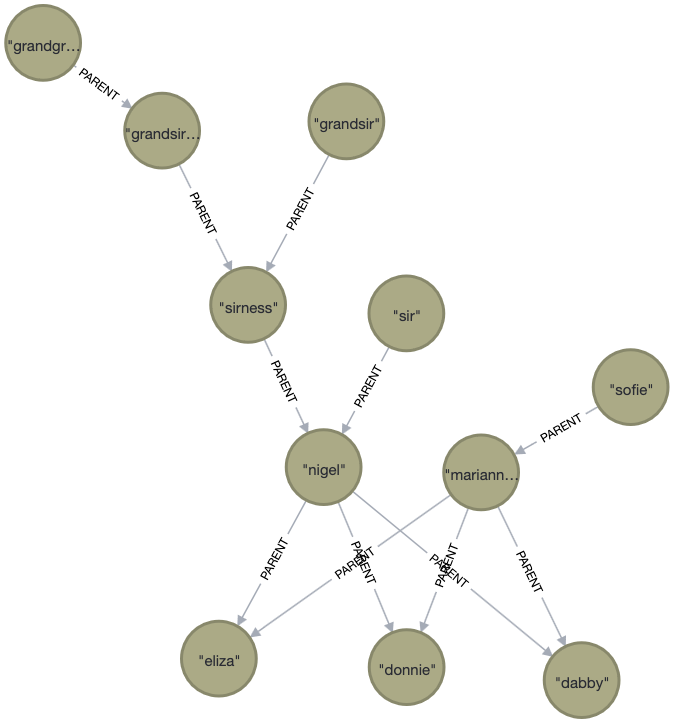
\includegraphics[width=0.9\linewidth]{graph}
    \caption{Граф родственников}
    \label{img:parents}	
\end{figure}

\section{Сравнение запросов в Neo4j и Prolog}

\subsection{Поиск родителей}

\subsubsection{Prolog}
\begin{lstlisting}[label=div,caption=Запрос]
parent(human(Who, _), human(eliza, _).
\end{lstlisting}

\subsubsection{Neo4j}
\begin{lstlisting}[label=div,caption=Запрос]
MATCH (child:Person)<-[:PARENT]-(parent:Person)
WHERE child.name = 'eliza'
RETURN parent.name, parent.gender
\end{lstlisting}


\subsection{Поиск братьев/сестер}

\subsubsection{Prolog}
\begin{lstlisting}[label=div,caption=Запрос]
sibling(Name1, Name2) :- parent(human(Mother, f), human(Name1, _)), 
	                     parent(human(Mother, f), human(Name2, _)),
	                     parent(human(Father, m), human(Name1, _)), 
	                     parent(human(Father, m), human(Name2, _)).

sibling(eliza, Who).
\end{lstlisting}

\subsubsection{Neo4j}
\begin{lstlisting}[label=div,caption=Запрос]
MATCH (child1:Person)<-[:PARENT]-(parent1:Person)
MATCH (child2:Person)<-[:PARENT]-(parent1:Person)
MATCH (child1:Person)<-[:PARENT]-(parent2:Person)
MATCH (child2:Person)<-[:PARENT]-(parent2:Person)
=WHERE parent1.gender = 'male' AND parent2.gender = 'female' AND child1.name = 'eliza' AND child2.name <> 'eliza'
RETURN child2.name, child2.gender`
\end{lstlisting}

\subsection{Поиск партнеров}
Партнерами считаются люди, у которых есть общие дети.

\subsubsection{Prolog}
\begin{lstlisting}[label=div,caption=Запрос]
partner(Name1, Name2) :- parent(human(Name1, _), Child), parent(human(Name2, _), Child), Name1 <> Name2, !.

partner(marianna, Who).
\end{lstlisting}

\subsubsection{Neo4j}
\begin{lstlisting}[label=div,caption=Запрос]
MATCH (child:Person)<-[:PARENT]-(parent1:Person)
MATCH (child:Person)<-[:PARENT]-(parent2:Person)
WHERE parent1.name <> parent2.name AND parent1.name = 'marianna'
RETURN DISTINCT parent2.name, parent2.gender`
\end{lstlisting}

\subsection{Поиск бабушки N-ого порядка}

\subsubsection{Prolog}
\begin{lstlisting}[label=div,caption=Запрос]
grandN(Grand, Child, 0) :- parent(human(Grand, _), human(Child, _)).
grandN(Grand, Child, N) :- N1 = N - 1, parent(human(Grand, _), human(Parent, _)), grandN(Parent, Child, N1).
	
grandmotherN(Grand, Child, N) :- gender(Grand, f), grandN(Grand, Child, N).

grandmotherN(Who, eliza, 2).
\end{lstlisting}

\subsubsection{Neo4j}
\begin{lstlisting}[label=div,caption=Запрос]
MATCH (grand:Person)-[:PARENT*2]->(child:Person)
WHERE child.name = 'eliza' AND grand.gender = 'female'
RETURN grand.name, grand.gender
\end{lstlisting}

